\documentclass[twoside,openright,a4paper,11pt,french]{article}
\usepackage[utf8]{inputenc}
\usepackage[french]{babel}
\usepackage[T1]{fontenc}
\usepackage{emptypage}

% Utilisation d'url
\usepackage{url}
\urlstyle{sf}

% Utilisation d'images, stockées dans le répertoire ./pics/
\usepackage{graphicx}
\graphicspath{pics/}

% Définition des marges
\usepackage{geometry}
\geometry{
  left=25mm,
  right=25mm,
  top=25mm,
  bottom=25mm,
  foot=15mm
}

\begin{document}

\pagestyle{plain}

% La page de garde
\thispagestyle{empty}

\begin{center}
       \noindent
       
\includegraphics[height=2.5cm]{./pics/uds.eps}       
       
       \vfill\vfill

    {\large \textsc{Licence 3 de Sciences, mention Informatique}}

    \bigskip\bigskip

    {\large \textsc{Réseaux et Protocoles}}

    \vfill\vfill

% Titre du document
    {\huge \sc
      \begin{center}
		Modèle de document\\pour un rapport d'étude
      \end{center}}

    \vfill\vfill

    {\large Présenté par}

\medskip

% Identité des auteurs
    {\large Julien \textsc{Montavont}}

% Contact mail
    {\small \url{montavont@unistra.fr}}

\bigskip

\end{center}



% La table des matières
\parskip=0pt
\tableofcontents

\section{Introduction}
\label{sec:intro}

Dans les réseaux locaux, les machines peuvent communiquer directement les unes
avec les autres par le biais d'un lien physique.\footnote{Ce lien peut directe
de machine à machine, ou indirecte: passant par d'autre équipement (switch,
hub,...).} En revanche, établir un lien entre des machines sur des réseaux
différents n'est pas aussi facile, cela pose en effet deux problèmes majeurs:
\begin{itemize}
\item Deux réseaux différents n'utilisent pas forcement la même technologie
pour transmettre des données au niveau protocolaire ou du lien physqiue.
\item Comme les machines ne sont pas physiquement sur le même réseau, il faut
un système d'adressage afin qu'une machine puisse joindre une autre machine
située dans un réseau différent, peu importe sa localisation.
\end{itemize}
Dans le cadre d'une communication, il est souvent pratique de diviser les
fonctionnalités nécessaire à l'échange d'information.  Pour cette raison il est
utile de définir un modèle théorique pour séparer les différentes tâches.
Aujourd'hui le standard en terme de modèle de communication est le modèle OSI
({\it Open Systems Interconnection}), qui divise en 7 couches les
fonctionnalités en question.

\bigskip
Le problème relatif à l'interconnection des réseaux (vu plus haut) est traité
par la couche 3 (nommé couche réseau) du modèle OSI.
Cette couche peux être fonctionnellement mise en oeuvre par le protocole IPv4.
C'est actuellement le protocole réseau (relative à la couche 3 du modèle OSI)
le plus utilisé et qui à permit le déployement massive d'Internet dans le
monde.\\
Dans la suite de ce rapport, nous allons étudier le fonctionnement d'IPv4, les
possibilités qu'il offre et l'écosystème de protocoles qui gravitent autour
d'IPv4 et qui sont nécessaires à son bon fonctionnement.  Nous allons commencer
par explorer le contexte de création de ce protocole et comprendre les
motivations qui ont pousser le concevoir.





% ------------------------------------------------

La technique de classe d'adressage IP ( classful network ) est une méthode utilisée de 1981 à 1993 pour allouer des adresses IPV4. Il a été défini en 1981 qu'une adresse IP est divisée en deux parties : une partie qui sert à identifier le réseau et une partie qui sert à identifier une interface sur ce réseau.
Dans cette méthode une adresse IP est divisée en 5 plages d'adresses IP et sont appelées classes. Ils sont organisés comme dans le tableau ci-dessous  :

\includegraphics{./pics/tableau.eps}


Chaque classe a un certain nombre d'octets servant à identifier le réseau. Une adresse IP de classe A à un identificateur de réseau sur 1 seul octet. Une adresse IP de classe B sur 2 octet et une de classe C sur 3 octets. Les adresses IP de classe D et E correspondent à des adresses IP particulières.
Les réseaux des différentes classes utilisent un certain nombre d'octets pour identifier le réseau. Ils ont donc un nombre différent d'octets restants qu'ils peuvent donner à des interfaces. 
Pour déterminer à quelle classe appartient une adresse IP il suffit de regarder les premiers bits de l'adresse.
Afin d'avoir un niveau supplémentaire, grâce auquel on gagne en flexibilité et en efficacité dans l'attribution d'adresse à l'intérieur d'une classe, on a introduit le concept de sous-réseau. Celui-ci introduit un nouveau numéro entre le numéro de réseau et le numéro d'hôte. Grâce aux sous-réseaux on peut par exemple diviser une adresse de classe B en 256 sous-réseaux pouvant chacun avoir 256 interfaces connectées.
On utilise un masque de sous-réseau pour obtenir la partie réseau de l'adresse IP. Le masque de sous-réseau est obtenu en mettant tous les bits de la partie réseau à 1 et tous les bits de la partie interface à 0. Lorsque deux adresses IP appartiennent au même sous-réseau, elles ont en commun les bits identifiants ce sous-réseau. Pour déterminer si 2 interfaces appartiennent au même sous-réseau, on les compare donc d'abord au masque de sous-réseau puis on les compare entre elles.
Cependant, ce système d'adressage a un grand inconvénient. En effet, il n'existe que 4 classes différentes et donc 4 types de réseaux de taille différentes. Cela conduit souvent à de grand gaspillage d'adresse. Par exemple, lorsqu'une entreprise souhaite une adresse IP. Si celle-ci possède 2000 interfaces, une adresse de classe C (2⁸ hôtes possibles) ne sera pas suffisante. Une adresse de classe B sera par contre largement trop grande (2¹⁶ hôtes possibles). C'est à cause de ce problème de gaspillage et du manque d'adresses IP que l'on est passé au   Classless InterDomain Routing (CIDR).

% ------------------------------------------------


\section{Concepts et utilisation}

Des données transmisent en utilisant le protocole IPv4 sont encapsulées dans un message que
l'on appelle un paquet IPv4. Ces paquets sont constitués d'un entête suivis des données à transmettre.

% Mossi
\subsection{Adresse IPv4}

L'entête contient des informations essentielles pour la transmission d'un paquet, notamment les
adresses source et destination.

Une adresse IP sert à identifier une machine (et plus précisément une des interfaces de cette machine)
dans un réseau particulier.
Comme nous le verrons plus tard cet identifiant unique permet de désigner à la fois un
réseau et une machine précise au sein de ce réseau.
Une adresse est codé sur 32 bits ce qui permet de coder 2\^32 soit 4294967296 adresses différentes.
Par convention on peut représenter une adresse IPv4 comme une suite de 4 nombres décimaux séparés par des points,
chacun traduisant un octet. Cette représentation a contribué à simplifier l'utilisation et la manipulation
des adresses.
Comme chaque nombre représente un octet, les valeurs de celui-ci sont comprises entre 0 et 255.

\vspace{1cm}
Exemple: adresse à valeur décimale: 212.217.0.1 => correspond sous sa forme
binaire à: 11010100.11011001.00000000.00000001
\vspace{1cm}

\subsubsection{Notion de NET ID et HOST ID}
Une adresse IPv4, en tant qu'identifiant d'une machine dans un réseau, contient deux informations:
une première partie qui identifie le réseau appelé NET ID (les bits de poids fort), une seconde qui identifie l’hôte appeler host-ID (les bits de poids faible).
Les machines qui se trouvent donc sur le même réseau partage le même NET ID pour leur adresse.

La longueur de ces deux parties est variable: la taille du HOST ID dépend de la taille du NET ID. Pour représenter la longueur de ces différentes parties on a introduit la notion de masque

\subsubsection{Masque de réseau}

Le masque sert à représenter la scission entre le NET ID et le HOST ID.
Il est codé sur 32 bits et adopte la même représentation qu'une adresse IP, à savoir
4 nombres décimaux séparé par des points.
La position des bits à 1 dans le masque corresponde à la position des bits définissant le NET ID dans l'adresse IP.
Pour obtenir les bits du NET ID il suffit de faire un ET logique entre l'adresse et son masque. Tous les autres bits (donc les bits à 0)
feront donc partie du HOST ID.
Les bits à 1 sont contiguës et commencent au bit de poids fort: le nombre de bit à 1 dans le masque, donne
le nombre de bit faisant partie du NET ID en partant du bit de poids fort dans l'adresse.

En conséquence plus le nombre de bit à 1 dans le masque est grand, plus le NET ID sera grand, et plus le HOST ID sera petit, car il restera moins de bit pour définir le HOST ID (la somme des deux devant évidemment faire 32 bits).

\begin{figure}[h]
\centering
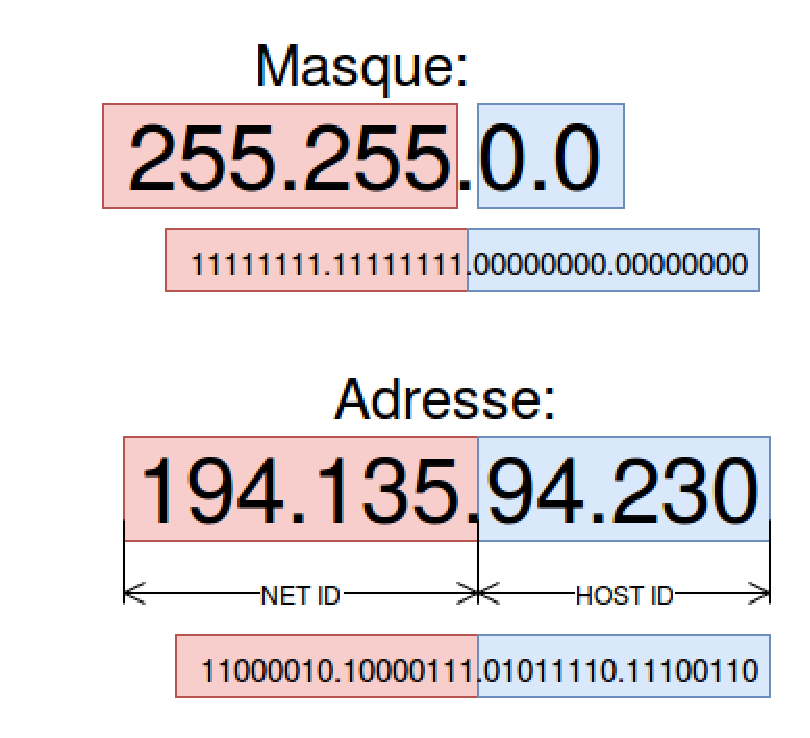
\includegraphics[width=7cm]{./pics/maskipv4.eps}
\caption{Example de masque de réseau.}
\label{fig:exmask}
\end{figure}

//TODO exemple
//TODO exemple invalide

\subsubsection{Classes d'adresse IP}
La technique de classe d'adressage IP ( classful network ) est une méthode
utilisée de 1981 à 1993 pour allouer des adresses IPV4.
Historiquement les classes d'adresse IP correspondaient à une plages d'adresses avec un masque figer pour une classe donnée.
Ce système permettait de déduire le masque en fonction
de l'adresse IP étant donné que chaque classe avait son masque défini de manière standard.
Il fut décrit dans le RFC 791\cite{url-RFC-791}.

Selon ce principe, chaque adresse IPv4 peut appartenir à une des 5 plages
d'adresses (appelées classes):

\begin{table}[h]
  \centering
% On paramètre ici le placement du texte dans les cases, en mode paragraphe de 5cm de large dans la case de gauche ("p{5cm}") et automatique avec un alignement à droite dans la case de droite ('r')
  \begin{tabular}{| p{5cm} | p{5cm} | r |}
    \hline
    \textbf{Classe} & \textbf{Masque reseau} & \textbf{Adresses}\\
    \hline
    A & 255.0.0.0 & De 0.0.0.0 a 127.255.255.255\\
    \hline
    B & 255.255.0.0 & De 128.0.0.0 a 191.255.255.255\\
    \hline
    C & 255.255.255.0 & De 192.0.0.0 a 223.255.255.255\\
    \hline
    D & 240.0.0.0 & De 224.0.0.0 a 239.255.255.255\\
    \hline
    E & Non defini & De 240.0.0.0 a 255.255.255.255\\
    \hline
  \end{tabular}
  \caption{Classes IPv4}
  \label{tab:classes}
\end{table}

A partir de ce tableau nous pouvons voir qu'il suffit de regarder les 4 bits de
poids fort pour déduire à quelle classe appartient une adresse.  Par exemple si
une machine à pour adresse 152.123.87.45 on sait en regardant les 4 premiers
bits que cette adresse fait partie de la classe B (car l'adresse commence par
10). De là, la machine n'a pas besoin de masque en plus car elle sait que le
masque correspondant un adresse de classe B est 255.255.0.0 .

Chaque classe à un certain nombre d'octets servants à identifier le réseau. Une
adresse IP de classe A à un identificateur de réseau sur 1 seul octet. Une
adresse IP de classe B sur 2 octet et une de classe C sur 3 octets.

Ce système permet donc d'adresser de nombreux réseaux avec un nombre de machine
variable en fonction de la classe, et tout cela sans avoir besoin de
communiquer ou de paramétrer un masque; celui-ci étant normalisé pour chaque
classe.  

Cependant il a un gros inconvénient, étant donné que les masques sont
figés, un réseau peut ne pas utiliser une partie plus ou moins importante
de ses adresses. Par exemple si un réseau contient 500 machines, il ne peut pas
utiliser d'adresse de classe A étant donné que celles-ci ne permettent d'avoir
que des réseaux de 254 machines maximum. Il va donc falloir utiliser des
adresses de classe B minimum, car elles permettent d'adresser 65534 machines au
sein d'un réseau\footnote{
De ce fait on remarque que la distribution de l’espace d’adressage entre
classes n'est pas homogène: la classe A a possédée 50\% de l’espace
d'adressage engendrée par les classes, la classe B 25\% , la classe C 12,5\%  et
les classes D et E 6,25\%.}. Nous pouvons donc utiliser 500 adresses sur les 65534
disponible, mais le reste sera "perdu".  Ce système était simpliste mais
n'était pas utilisable sur le long terme car il "gâche" des adresses en
n'utilisant pas tout son espace d'adressage.

Afin d'avoir un niveau supplémentaire, grâce auquel on gagne en flexibilité et
en efficacité dans l'attribution d'adresses à l'intérieur d'une classe, on a
introduit le concept de sous-réseau. Celui-ci correspond à couper la plage
d'adresses appartenant a un bloc d'une classe en plusieurs réseaux. Grâce aux
sous-réseaux on peut par exemple diviser une adresse de classe B en 256
sous-réseaux pouvant chacun avoir 256 interfaces connectées. 


\subsubsection{CIDR}

Aujourd'hui le système le plus utilisé est CIDR (Classless Inter-Domain
Routing) remplace le système de classe d'adresse. CIDR permet de créer des
masque beaucoup plus fin, étant donné qu'on n'est plus limité à des masque de
réseau fixe, on peut ajuster le masque pour avoir le nombre de machine
adressable dans un réseau le plus proche possible du nombre de machine que l'on
souhaite adressé.  Cela permet de limiter les pertes en adresse inutilisé, si
la plage est correctement découpée.  On peut donc créer des masques à la
séparation entre le NET ID et le HOST ID se trouve n'importe où, même en plein
milieu des octets (ce qui était impossible avec les classes d'adresse), ce qui
apporte une plus grande flexibilité.  Cela permet aussi de créer une hiérarchie
dans une plage d'adresse réseau qui serait découper en plusieurs réseaux
"fils", et cela permet notamment, avec cette hiérarchie, de réduire la table de
routage des routeur.  De là est né une nouvelle notation des masques: on écrit
le nombre de bit à 1 dans le masque à la suite de l'adresse IP et séparé par un
slash.


\begin{figure}[h]
\centering
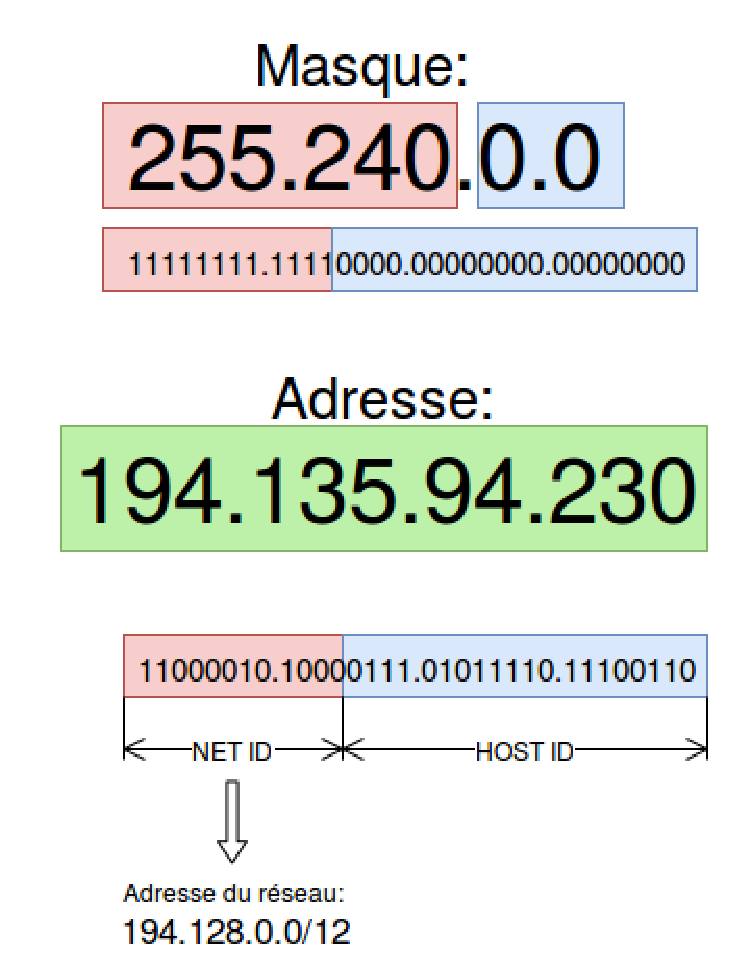
\includegraphics[width=7cm]{./pics/maskipv4cidr.eps}
\caption{Example de masque utilisant le systeme CIDR.}
\label{fig:exmask}
\end{figure}


\subsubsection{Types d'adresses}
La variété des exigences en matière de réseaux a donnée lieu à une
classification progressive des adresses selon des rôles bien précis. En effet,
pas toutes les adresses IPv4 ont la même signification: à certaines adresses
(ou plages d'adresses) ont été attribué par convention des fonctions ou des
caractéristiques particulières.  Dans la suite de cette partie nous analyserons les
adresses IP sous trois aspects différents: nous classifierons d'abord les adresses selon
le type de diffusion qu'elles permettent d'effectuer, puis nous introduirons le
concept d'adresse publique et d'adresse privée, enfin nous parlerons de l'utilisation
particulière qui a été faite avec certaines adresses.



\paragraph{Mode de diffusion}
Dans le cadre des transmissions, en plus de communiquer entre deux interfaces, il est 
parfois nécessaire qu'un message soit reçu par un groupe de machines ou que 
même la totalité du réseau reçoivent ce message.

On a défini pour cela plusieurs types de diffusions associés à certaines adresses particulières.

Le type de diffusion le plus utilisé est la diffusion en unicast. Dans ce mode,
l'adresse IP désigne une machine de manière unique. L'adresse IP appartient
à une seule machine et sert à l'identifier sur un réseau.  C'est le type
d'adresse que nous avons abordé jusqu'à présent.  Mais il peut être intéressant
de pouvoir contacter plusieurs machines en même temps. On pourrait bien sûr
envoyer des paquets en unicast à chaque machine que l'on souhaite contacter,
mais cela serait fastidieux et inonderait le réseau inutilement. Une solution plus
pratique est d'avoir une adresse qui désigne plusieurs machines à la fois. Cela
permet d'envoyer un seul paquet qui est remis à plusieurs machines. Il
existe pour faire cela plusieurs types de diffusion.
\begin{itemize}
\item Le broadcast: Ce mode de diffusion permet d'envoyer un paquet unique tout en 
joignant toutes les machines sur un réseau. Lorsque les machines reçoivent ce
paquet, elles s'aperçoivent que l'adresse de destination du paquet est l'adresse de
broadcast et elles vont alors traiter le paquet. L'adresse de broadcast d'un réseau
est défini comme la plus "haute" adresse du réseau: cela se traduit par la mise
à 1 de tous les bits de la partie HOST ID. Cette adresse ne peut donc pas être
attribuée à une machine en tant qu'adresse unicast.  Le broadcast est utilisé
par des protocoles tel que ARP et DHCP.  Nous pouvons remarquer qu'avec cette
définition, nous pouvons envoyer un message de broadcast à n'importe quel
réseau, incluant le notre. En réalité (sauf
configuration volontaire) les routeurs ne laissent pas passer les messages de
broadcast d'un réseau à un autre; excepté quelques cas spéciaux comme DHCP où un
serveur peut s'adresser à plusieurs réseaux, et où ses messages de broadcast
peuvent être relayés par les routeurs (appelés DHCP agents).
\item Multicast: Ce mode de diffusion permet d'envoyer un paquet à destination
de plusieurs machines. L'adresse IP multicast sera donc vu comme l'adresse d'un groupe
mutlicast, qui désigne donc plusieurs machines. Pour qu'une machine fasse partie d'un
groupe multicast, il faut qu'elle s'abonne à ce groupe: cela veut dire que si elle reçoit
un paquet avec comme adresse de destination l'adresse du groupe multicast, elle va traiter
le paquet.
Bien entendu les membres d'un même groupe ne sont pas obligés d'être sur le même réseau. Dans ce
cas les machines doivent indiquer à leur routeur qu'il existe un ou plusieurs groupe multicast et celui-ci deviendra alors un routeur multicast 
 Le protocole IGMP va entrer en jeu pour faire cet échange.
Cette indication a été rendu obligatoire dans le but de ne pas faire circuler tous les paquets a destination de groupes multicast.
 Il n'est en effet pas nécessaire de relayer tous les paquets de tous les groupes
multicast sur le réseau, si celui-ci ne contient aucun abonné au groupe.
Le faite d'avertir le routeur qu'il y a des machines abonnées à un groupe dans le réseau permet aussi à celui-ci
d'établir un lien avec l'émetteur. Mais ceci fait partie du routage des paquets par le routeur.
Il existe une plage d'adresse qui est réservée pour les adresses IP multicast. Lorsqu'on veut contacter
plusieurs machines, une adresse dans cette plage peut être utilisée.
Elle s'étend de l'adresse 224.0.0.0 à l'adresse 239.255.255.255 et a pour masque 240.0.0.0 . Cela laisse donc 2\^28 adresses
multicast différentes.
Au sein de cette plage d'adresse il existe une catégorisation:
//TODO
\begin{itemize}
\item
\end{itemize}
Ce mode permet de limiter le nombre de paquets envoyés pour joindre plusieurs machines et il est très utilisé dans le cas
de diffusions en streaming ou de vidéoconférences, où il faut faire parvenir une même information à plusieurs participants.

\item Anycast: Une adresse anycast, tout comme les adresse multicast, identifient plusieurs machines. La différence avec multicast
est qu'en mode de diffusion anycast, la paquet ne va pas être remit à tous les membre du groupe, mais seulement à un seul (le premier qui le réceptionne).
Le choix de la destination et le routage à adopter se base sur plusieurs critères telles que la "distance" avec la machine, la disponibilité,
la charge, ... . Cela permet d'avoir des systèmes toujours disponible même en cas de forte charge, en repartissant celle-ci sur
plusieurs machines.
\end{itemize}



\paragraph{Adresses publiques et adresses prive}
L'expansion exponentielle d'Internet a posé, seulement quelques années après sa création, des
soucis de pénurie d'adresses. Plusieurs mesures ont été prises pour limiter la
portée de ce problème. Malgré ça, le stock d'adresses IPv4 non réservée
est malheureusement épuisé depuis le 2011.

Une des dispositions les plus connues et efficaces a été la création du concept
d'adresses privées. Le RFC 1918 introduit la notion d'adresses privées: une adresse
appartenant à cet catégorie est un identifiant unique dans un réseau (ou sous
réseau) mais il ne comporte aucune contrainte d'unicité dans l'échelle globale
(Internet). L'idée derrière la conception des adresses privées était celle d'
avoir des identifiants qui peuvent être utilisés lorsque une machine n'a pas
pas besoin de communiquer avec des interfaces au-delà de son réseau.

A ce titre des plages d'adresses ont été réservées pour cet usage:

\begin{itemize}
\item Un bloc d'adresses appartenant a la classe A: \textbf{10.0.0.0/8}
\item 16 blocs d'adresses appartenant a la classe B: \textbf{172.16.0.0/12}
\item 256 blocs d'adresses appartenant a la classe C: \textbf{192.168.0.0/16}
\end{itemize}

\smallbreak
Le concept d'adresses privées s'oppose à celui d'adresses publiques: ce dernier est 
une adresse unique sur Internet et est en conséquence atteignable par n'importe
quel hôte sur Internet.

Aujourd'hui des systèmes comme celui de la NAT ({\it Network Address
Translation}) permettent à des machines ayant des adresses IP privée de communiquer
de manière transparente avec des hôtes en dehors de leur réseau. Ce système est
largement utilisé dans les réseaux domestiques pour permettre aux machines au
sein de ceux-ci d'être directement connecté à Internet. On parlera plus en
détail du NAT dans la section %TODO \ref{} %.
\smallbreak


 
L'augmentation des difficultés relatives à la procédure de réservation des adresses
publiques au sein des organisme responsables des allocations\cite{url-RFC-1918}
(tels que le IANA) ont contribués a promouvoir l'utilisation des adresses privées à la place
 des adresses publiques lorsque cela est possible.
L'utilisation des adresse privées a pour conséquence la préservation des plages
d'adresses IP publiques, ce qui constitue un avantage certain: l'utilisation
des adresses privées permet d'éviter le gaspillage des adresses publique là ou elles
ne sont pas nécessaires.


\paragraph{Adresses speciales}
L'usage spéciale d'une adresse IP découlait de l'émergence
%TODO (apparition??) 
d'un nouveau besoin dans le domaine des réseaux; c'est pour
ça que jusqu'à 2002, l'attribution des rôles spéciaux des adresses
IPv4 était présentés dans divers document, qui présentaient, et répondaient à chaque fois à une
problématique bien particulière. Le RFC3330 est un des premiers documents à
rassembler les classification des adresses IPv4 selon leur rôles et significations.

%TODO lien%

\begin{description}
\item[0.0.0.0/8]
Cette plage d'adresses indique la machine courante dans le réseau courant.
Les adresses dans cette plage sont notamment utilisées dans certains protocoles de
configuration comme adresse source, lorsqu'une machine n'a pas encore d'adresse effective.
%RFC 1122 %

\item[127.0.0.0/8]
Une adresse appartenant a ce bloc est dénommée adresse de {\it loopback}.  Un
paquet envoyé vers une telle adresse retourne directement chez l'expéditeur, sans sortir
du contexte de la machine émettrice. Parmi les adresses de cette plage,
127.0.0.1 est celle utilisée le plus fréquemment\footnote{Comme l'indique
le RFC 1122, certaines implémentations de l'adresse de {\it loopback} se
limitent à utiliser le bloc 127.0.0.1/32, ce qui se traduit par l'unique utilisation de
l'adresse 127.0.0.1 }: dans plusieurs contextes cet adresses est référencée par
l'alias "{\it localhost}".\footnote{La correspondance entre le nom {\it localhost} et
l'adresse 127.0.0.1 est généralement mise en place par le système d'exploitation.
Dans les systèmes de type UNIX une entrée reliant ces deux entités est généralement
présente dans le fichier "/etc/hosts".}
Une adresse de {\it loopback} n'a pas de sens en dehors
d'une interface même, et c'est pour cela qu'elle ne devrait apparaître à aucun moment dans le réseau.

%RFC 1122 %

\item[169.254.0.0/16]
Cet plage d'adresses a été désignée comme contenant les adresses qu'on appelle
de {\it lien local}.  Les adresses dites de {\it lien local} sont utilisée lorsqu'une 
machine n'a aucun moyen d'obtenir une adresse IP (par exemple par le biais
d'un serveur DHCP ou simplement avec une configuration manuelle).  L'obtention
d'une adresse de {\it lien local} est faite de façon automatique à travers un
processus d'auto-configuration souvent appelé par l'acronyme APIPA ({\it
Automatic Private Internet Protocol Addressing}) ou par le nom IPv4LL.  Le
fonctionnement du processus APIPA (décrit dans le RFC 3927) est assez complexe
 et entraîne l'utilisation de certaines fonctionnalités du
protocole ARP (qu'on traitera plus en détail dans la section %TODO \ref{sec:suiteproc} % )
. Son fonctionnement peut être synthétisé dans ses grandes lignes par la démarche suivante:

\begin{description}
\item[Sélection de l'adresse]
La machine choisit aléatoirement
    \footnote{Il est conseillé d'utiliser l'adresse MAC de l'interface en question
    pour générer l'adresse de {\it lien local} pour qu'il y ait une plus forte chance
    qu'elle soit unique dans le réseau.} 
une adresse appartenant à la plage 169.254.0.0/16

\item[Sondage sur l'adresse]
Une fois qu'on a sélectionné une adresse, il faut s'assurer que la même adresse ne soit
pas déjà utilisée par d'autres machines sur le réseau. Dans ce but la machine
pose la question à toutes les autres machines du réseau au moyen d'un ou plusieurs messages
en brodcast, et attend une réponse pendant un certain intervalle de temps\footnote{
Des précautions sont prises pour éviter les conflits générés par plusieurs
machines qui effectuent simultanément cette action pour la même adresse,
notamment: des intervalles de temps aléatoires entre l'envoie des messages et la mise
en place d'une écoute active des autres messages pendant le temps de l'enquête.}
L'absence de réponse indique que l'adresse est bien unique. Si l'adresse n'est
pas unique il faut en choisir une autre.

\item[Annonciation de l'adresse]
A ce point la machine peut communiquer aux autres machines l'adresse qu'elle
vient de réserver.

\end{description}



Ce processus est basé sur le concept de {\it Zeroconf}: il permet la mise en
place d'un réseau IPv4 sans aucune configuration. Ce type de système,
C'est aussi grâce a ce genre de systèmes, qu'on 
pourrait synthétiser par la devise %TODO slogan??  
"plug and play", que le concept de Networking (et avec lui Internet) a pu se
diffuser assez rapidement: grâce à APIPA un réseau IPv4 peut être facilement
mis en place sans le besoin d'aucune connaissance technique.\\

La plage d'adresses 169.254.0.0/16, désigne une plage d'adresse privée: les
adresses de type {\it lien local} ne sont donc pas atteignables en dehors de
leur réseau de définition. 
Cette plage d'adresses pose par contre des limites par rapport aux autres
plages d'adresses privée car, à la différence des autres, elle ne peut pas être
divisée en sous réseaux\footnote{Ce qui est assez logique si on considère que
le processus d'obtention d'une adresse de {\it lien local} (APIPA) utilise
les liens "physiques" entre les machines pour communiquer, et il ne peut
 considérer aucune notion de sous-réseau.}
: en effet un paquet destiné à une adresse de {\it lien local} ne doit pas être
retransmise par un hôte intermédiaire.\footnote{Dans le paquet destiné
a une adresse de {\it lien local} le champ TTL est usuellement mis a 1
pour empêcher des forwarding.}

\item[192.88.99.0/24]
Les adresses appartenant à ce bloc désignent des routeurs 
fournissant un service de type {\it 6to4}. Ce type de service
permet de relier des réseaux IPv4 avec des réseaux IPv6.
Les adresses dans cette plage sont traitées comme étant des adresses
de type {\it anycast}.


\end{description}







%Victor
\section{Suite de protocole}

\subsection{ARP}
ARP (Address resolution protocol) est un protocole à cheval entre la couche 2 et
la couche 3 permettant de faire la conversion entre les adresses de niveau 2 et de niveau 3.
Cela est très utilisé étant donné que les hôte connaissent souvent les adresses IP de leur destinataire,
mais rarement l'adresse de niveau 2 de ce destinataire ou de la passerelle à contacter pour joindre
le destinataire.

\subsubsection{Cache ARP}
Le cache ARP ou table ARP est une table sotcké en local par un hôte et qui ressence les associations entre adresse IP et adresse MAC.
Ces associations peuvent être soit de type statique, donc écrite "en dur" par l'administrateur, ou dynamique, donc issue d'échange de trame ARP,
et qui possèdent, en plus des associations statique, une durée de validité, étant donné qu'une interface peut changer d'adresse IP et qu'il vaut
maintenir la table à jour.
Cette table peut donc être représenté comme une suite d'entrés, contenant chacune une adresse IP, une adresse MAC et éventuellement une durée de vie.

\subsubsection{Entête}
//TODO


\subsubsection{Fonctionnement}
Prenons l'exemple où A veux envoyer un message à B. A connait l'adresse IP de
B. Donc A va préparer son paquet qu'il va envoyer à B, avec son adresse IP en
source et l'adresse IP de B en destination. La paquet passe dans la couche
liaison, il va être enpaqueté dans une trame de niveau 2. Cette trame aura
comme adresse source l'adresse de niveau 2 de A, mais à ce moment il ne peux
pas completé l'adresse destination de la trame: en effet, il ne connait
l'adresse de niveau 2 du destinataire. La paquet reste bloqué en couche 2 et ne
peux pas être envoyé au destinataire. Comment obtenir l'adresse de niveau 2 du destinaire?
Le protocole ARP est capable de faire cette translation.

Pour faire cela l'hôte A va tout d'abord regarder dans sa table ARP si il n'a pas une entrée pour l'adresse IP à laquelle il souhaite envoyer son paquet. Si il tourve une correpondance, il va utiliser l'adresse MAC stocker en correspondance avec l'adresse IP recherché.
Si il ne trouve pas de correspondance il va emmetre une trame ARPREQUEST pour tenter de contacter le possesseur de l'adresse IP qu'il souhaite contacter. Il va mettre dans cette trame (en plus de l'entête de niveau 2) un entête ARP. Celui-ci contient plusieurs informations:
//TODO quels info mettre? type de trame ARP: request ou reply
Les informations importantes pour permettre la résolution d'adresse sont les adresses IP source et destination, ainsi que les adresses MAC source et destination.
L'hôte A va donc mettre son adresse IP en IP source (entête ARP) et son adresse MAC dans l'adresse physique source (entête ARP). Dans le champ d'adresse IP destination (entête ARP) l'hôte A va mettre l'adresse IP de l'hôte qu'il veut contacter. Etant qu'il cherche à avoir l'adresse physique de l'hôte B, il ne peut pas indiquer d'adresse MAC dans le champ d'adresse physique destinataire. Ce champ est donc rempli avec la valeur 0.
Sachant que l'hôte A n'a pas l'adresse physique du destinataire, il va envoyer sa trame en broadcast pour espérer atteindre l'hôte B sans connaitre son adresse MAC.
Une fois que l'hôte B reçoit la requète ARP, il va analyser son entête et remplir sa table ARP avec l'adresse IP de l'hôte A et l'adresse physique de A. Cela permet de créer une correspondance entre l'adresse IP et MAC de A, pour non seulement pouvoir répondre à sa requête ARP, et pour pouvoir contacter A dans le futur sans avoir besoin de refaire la demande ARP.
Ensuite l'hôte B va répondre avec une trame ARPREPLY. L'entête est similaire aux ARPREQUEST, seul le champ indiquant s'il s'agit d'une trame ARPREQUEST ou ARPREPLY change. Dans cette trame, l'hôte B va placer son adresse IP dans le champ adresse IP source et son adresse physique dans le champ d'adresse physique source. Il va aussi mettre l'adresse IP de A dans le champ adresse IP destination et l'adresse MAC de A dans le champ d'adresse physique destination. Il va ensuite envoyer cette trame en unicast à A.
Lorsque A reçoit la trame ARPREPLY, il va à son tour mettre dans sa table ARP, la correspondance entre l'adresse IP source et l'adresse MAC source de la trame (soit les adresses de B).
Une fois cette association mise en place, le paquet IP que voulait envoyer A au début et mis en pause le temps que le protocole ARP fasse l'association, est enfin envoyé étant donné que A à maintenant l'adresse physique de B.

\subsubsection{ACD}
Le protocole ACD (Adresse conflict detection) permet, comme son nom l'indique, de détecter les conflits d'adresse, qui sont l'utilisation de la même adresse IP par deux ou plusieurs hôtes en même temps.
Pour ce faire il utilise le protocole ARP avec une succession d'étape permettant de garantir l'utilisation de manière unique d'une adresse IP.
Pour commencer, ACD intervient au moment où une interface reçoit une adresse IP (soit par DHCP, soit par une configuration manuelle,...). Il faut à ce moment vérifier si l'adresse proposer n'est pas déjà utlisé par un autre hôte sur le réseau.
L'hôte va alors émettre une requète ARP en broadcast en remplissant l'entête ARP avec son adresse MAC dans le champ d'adresse physique source et 0.0.0.0 dans l'adresse IP source (car il n'a pas encore d'adresse IP attribuer, et pour éviter de corrompre les table ARP des autre hôte). Le champ adresse IP destinataire est complété avec l'adresse que l'on souhaite acquérir. On ne peut pas remplir le champ d'adresse physique destinataire étant donné qu'on ne sait pas si il y a des hôte avec cette adresse déjà configuré.
Une requète ARP contenant 0.0.0.0 comme adresse IP source est appelé ARP probe car elle sert à "sonder" si un autre hôte utilise déjà l'adresse que l'on passe dans le l'adresse IP destinataire.

Après avoir attendu un temps pouvant aller jusqu'à 1 seconde, l'hôte va envoyer un nombre d'ARP probe compris entre 1 et 3, et tous espacé d'un intervalle compris entre 1 et 2 secondes.
Si dans un délai de 2 secondes après l'émission de l'ARP probe l'hôte reçoit un paquet ARP request ou reply avec comme adresse IP source l'adresse qu'il souhaite acquérir, alors cela veut dire qu'un autre hôte est entrain d'utiliser cette adresse. L'ARP reply peut être la réponse à l'ARP probe émis et l'ARP request peux simplement être une demande ARP faite par l'hôte qui utilise déjà l'adresse que l'on souhaite acquérir.
En plus de surveiller ces deux types de messages, l'hôte doit vérifier les message ARP probe qu'il reçoit. En effet, il se peut que deux hôte décide de configurer leur interfaces avec la même adresse au même moment. Sachant qu'aucune de ces deux interface n'a encore d'adresse IP attribuer, aucune ne va répondre à l'ARP probe deu deuxième hôte. Cela va conduire à l'attribution de la même adresse pour plusieurs interfaces. Pour éviter ce problème l'hôte doit surveiller les ARP probe qui passe à son interfaces. Si il en reçoit un avec comme adresse destination la même adresse qu'il souhaite acquérir mais avec une adresse physique différente de la sienne, cela veux qu'un autre hôte souhaite utiliser la même adress que lui.

\subsection{ICMP}
ICMP (Internet Control Message Protocol) est un protocole de niveau 3 faisant partie intégrante du protocole IPv4. Il permet de transmettre des informations de controle et d'erreur. Les messages ICMP sont empaquetés dans des paquets IP, ils diposent donc d'un entête de paquet IP. Cet entête est le même que pour tout les autres entêtes de paquet d'IPv4. Deux champs son intéressant dans le cas d'un paquet ICMP, les champs Protocol et Type of service. Le champ Protocol est mis à à la valeur 1 pour dire que le paquet contient un message ICMP, et le champ ToS est mis à 0 //TODO(pourquoi 0?)//.
Après le header du paquet IPv4, commence la partie data qui contient le message ICMP. Ce message contient des champs différent en fonction du type de message à passer. Cependant les trois premier champs sont toujours les mêmes.
Les types de messages ICMP qui vont suivrent sont décrit dans la RFC 792.\footnote{https://tools.ietf.org/html/rfc792}
\\
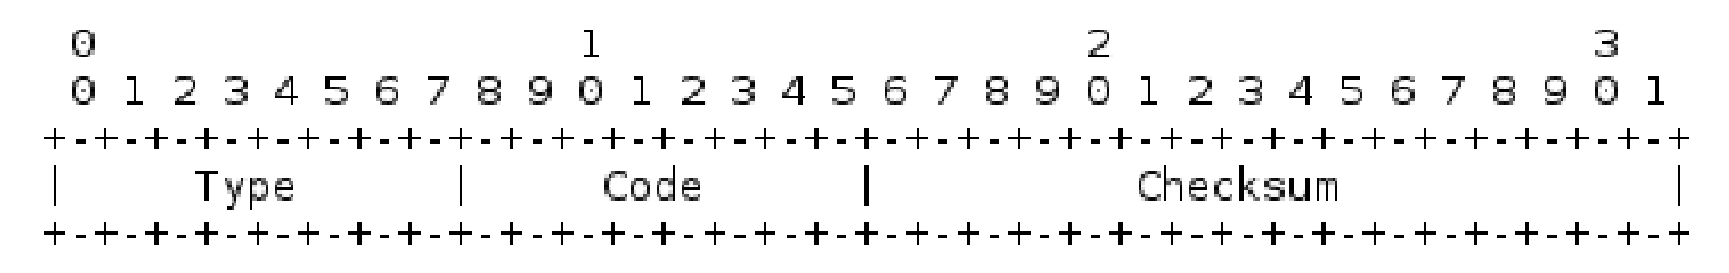
\includegraphics[width=15cm]{./pics/header.eps}
\\Le premier champ est celui de type. Il permet, premièrement, de donner le type du paquet et de l'information à transmettre, et deuxièmement de préciser la nature des champs qui vont suivres. En effet, comme vu plus haut, les messages contiennent des champs différents selon le type du message ICMP.
\\Le deuxième champ est le code. Il permet de subdiviser le type en donnant des détails plus précis.
\\Enfin le troisième champ est la somme de contrôle (checksum)//TODO(plage de controle).
\\Commençons avec les messages qui possèdent l'ensemble de champs le plus simple.

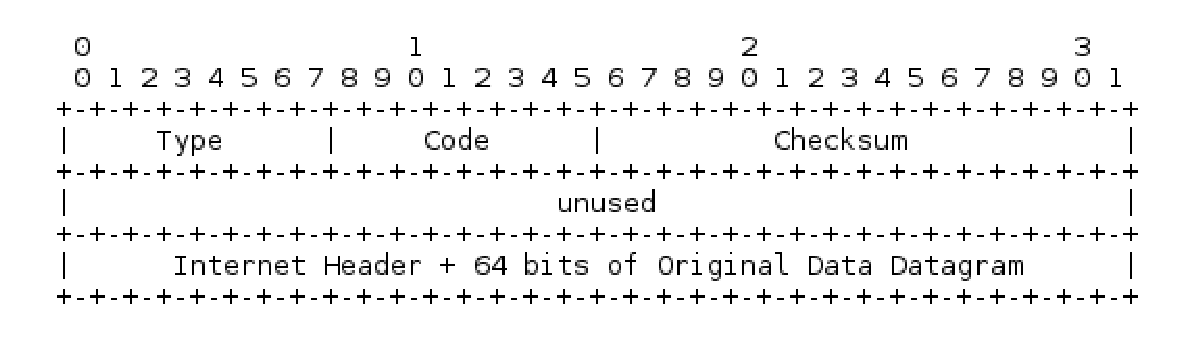
\includegraphics[width=15cm]{./pics/header1.eps}

\\Les messages qui utilisent cette organisation sont les messages de type 3, 4 et 11.

\subsubsection{Message de type 3: Unreachable Destination}
Les messages de type 3 sont émis lorsqu'un paquet n'a pas réussi à joindre la destination (Unreachable destination). Cette erreur peux être dut à plusieurs facteurs, et les codes permettent de préciser pourquoi le paquet n'a pas pu rejoindre sa destination.
\paragraph{Code 0}

\subsubsection{Message de type 4:}

\subsubsection{Message de type 11: Time Exceeded}
Ces messages sont envoyés lorsque le TTL d'un paquet à atteind 0. Une autre utilisation des ces messages est lorsque que le temps de ré-assemblage des fragments d'un paquet est dépassé. Ces deux cas sont distingé par le code. Ces messages ont pour destinataire l'hôte qui à envoyé le paquet qui à provoqué l'erreur.//TODO(vérifier)
Le champ Internet header contient l'entête du paquet qui a été supprimé plus les 64 bits suivant celui-ci. Cela permet à l'émetteur de retrouver quel paquet à été supprimé.
\paragraph{Code 0:}
Le code 0 est utilisé pour indiquer que le TTL du paquet posant problème est arrivé à 0. Lorsque le TTL d'un paquet arrive à 0, celui-ci est supprimer et un message ICMP de type 11 et de code 0 est envoyer par le routeur qui à détécté le problème. Cela permet principalement d'éviter qu'un paquet sans dans une boucle et qu'il soit rélayé à l'infini.
\paragraph{Code 1:}
Le code 1 est quant à lui utilisé pour indiquer //TODO


\subsubsection{Message de type 5:}
Les message de type 5 utilisent les entêtes ci-dessous et servent à faire de la redirection. En effet, lorsqu'un routeur détecte que le prochain routeur dans lequel va transiter le paquet se trouve dans le même réseau que l'émetteur de ce paquet, il va envoyer un message ICMP pour avertir cet hôte (et/ou le réseau) qu'il existe un chemin plus court en envoyant directement les paquets vers le prochain routeur. Ce message ICMP va avoir pour effet de modifier la table de routage interne à l'émetteur (et/ou des hôtes connecté au réseau). Concernant le paquet que le premier routeur à reçu, il va le transmettre vers sa destination.

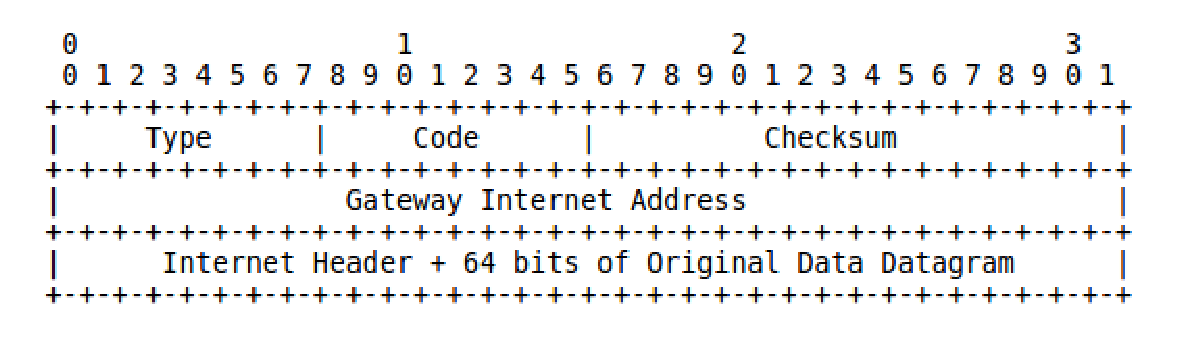
\includegraphics[width=15cm]{./pics/header2.eps}

\\
Le champ Gateway Internet Address contient la l'adresse du routeur auquel il faut faire transiter le traffique directement pour avoir un chemin de routage plus court.
Le champ Internet Header contient toujours l'entête du message ayant porvoqué l'envoie du message ICMP plus les 64 bits suivant l'entête. Cela permet à (aux) hôte(s) de pouvoir modifier leur table de routage en fonction la destination que cherchait à atteindre le paquet.
\paragraph{Code 0}
Ce code indique que la redirection est adresser à tout le réseau de l'émetteur du paquet.
\paragraph{Code 1}
Ce code indique que la redirection est adresser à l'émetteur du paquet.
\paragraph{Code 2}
Ce code indique que la redirection est adresser à tout le réseau de l'émetteur du paquet et aux services(//TODO(préciser)).
\paragraph{Code 3}
Ce code indique que la redirection est adresser à l'émetteur du paquet(//TODO(préciser)).

\\
\\
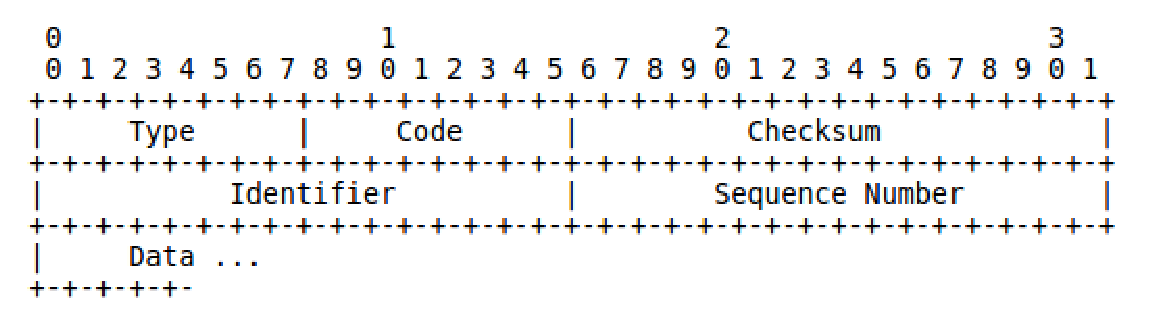
\includegraphics[width=15cm]{./pics/header3.eps}
\\

\subsubsection{Message de type 8 et 0:}
Les messages de type 8 et 0 servent à faire des envoies et des renvoies d'information. Ils utilisent pour cela l'entête ci-dessus. Les messages de type 8 font des envoies d'informations, appelé echo request. Tandis que les messages de type 0 sont envoyés en réponse aux echo request et renvoie les informations reçus de ceux-ci; ils sont appelés echo reply. Etant donnée que les echo reply sont des réponses aux echo request, l'adresse destination des echo reply est l'adresse source des echo request. Ces deux messages peuvent envoyés et reçu aussi bien par un hôte que par un routeur. Ce sont notamment les message envoyés par la commande {\it ping} qui permet de vérifier si l'on peux communiquer avec un hôte ou un routeur.
Les champs Identifier et Sequence Number aide l'émetteur de l'echo request à associer les echos request qu'il à envoyés avec les echos reply qu'il à reçus.
//TODO(qui a t-il dans data?)
\subsection{IGMP}


\subsection{DHCP}
\footnote{RFC 2131: https://tools.ietf.org/html/rfc2131}
Le protocole DHCP (Dynamic Host Configuration Protocol) sert à l'autoconfiguration des interfaces. Plus précisement, il  permet d'attribuer une adresse IP à une interface et de lui faire parvenir d'autres information essentielle pour le fonctionnement de l'interface sur le réseau.
Voyons comment une interface peut ce configurer aurpès d'un serveur DHCP.

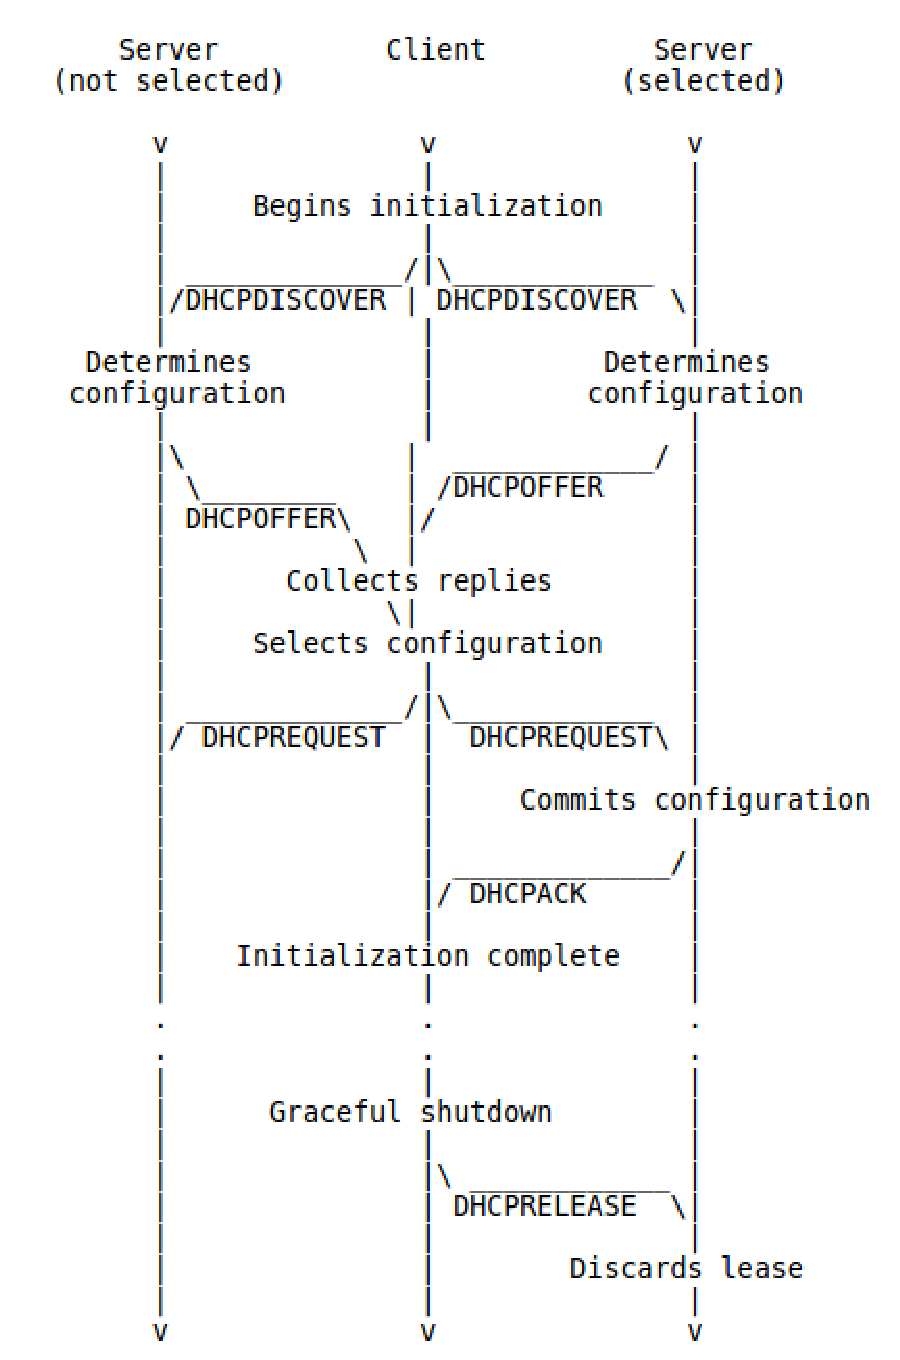
\includegraphics[width=6cm]{./pics/timeline_dhcp.eps}
\\
Lorsqu'une interface, qui n'a pas d'adresse IP, souhaite en recevoir une, elle va emettre un message DHCPDISCOVER en broadcast sur son réseau. Des agents DHCP peuvent faire passer ce message DHCP sur un autre réseau si le serveur DHCP (qui distribue les adresses) ne se trouve pas sur le même réseau que l'hôte qui fait la demande. L'hote va utiliser comme adresse IP 0.0.0.0.
\\Etant donnée que le message est envoyé en broadcast, tout les hôtes sur le réseau vont recevoir le message, et en particulier le ou les serveurs DHCP qui pourraient s'y trouver. Si cela est le cas, ceux-ci vont répondre avec un DHCPOFFER. Ce message contient entre autre l'adresse IP proposé pour le client souhaitant se configurer, ainsi que le masque de sous-réseau de l'adresse. A ce moment là l'adresse n'est pas encore attribuer et réservé pour l'hôte étant donnée qu'il peux refuser l'offre et accepter l'offre d'un autre serveur. Si jamais l'hôte ne reçoit aucun DHCPOFFER, il va ré-émettre un DHCPDISCOVERY. Si il reçoit un ou plusieurs DHCPOFFER, l'hôte va devoir choisir une configuration qui lui est proposé. Une fois ce choix fait, il va informé les serveurs DHCP de son choix à l'aide d'un message DHCPREQUEST émis en broadcast. Ce message va contenir l'identifiant du serveur DHCP retenu ainsi que la configuration souhaité par l'hôte (adresse IP et masque de sous-réseau). Ce message peut être interprété de deux manières différentes selon le serveur:
\item- si ce n'est pas le serveur retenu, il considère le message comme une déclinaison de l'offre.
\item- si c'est le serveur retenu, il va sortir l'adresse attribué l'hôte de la plage d'adresse libre pour ne plus l'attribuer à un autre hôte. Il va ensuite émmetre un message DHCPACK contenant la configuration effective de l'hôte avec notemment: l'adresse IP, le masque de sous-réseau, la durée du bail, l'adresse de la passerelle par défaut et l'adresse du serveur DNS.
Si pour quelque raisons le serveur n'est pas capable d'attribuer l'adresse proposé dans l'offre (par exemple si l'adresse à été attribuer entre temps), le serveur emet un DHCPNAK pour avertir l'hôte que l'adresse n'est plus disponible. L'hôte devra alors recommencer la procédure pour obtenir une adresse IP.
\\Enfin si le serveur ne reçoit pas de message DHCPREQUEST, la procédure s'arrêtrra à ce moment et l'adresse n'étant pas encore attribuer à l'hôte elle reste disponible pour être attribuer à d'autre hôte.
Arrive la dernière étape. Si le client reçois un message DHCPACK, il peux prendre en compte la configuration (adresse IP, masque de sous-réseau, DNS, passerelle par défaut et durée de bail). Il va effectuer une dernière vérification pour s'assurer que l'adresse qui lui à été attribué est bien unique sur le réseau pour éviter d'avoir deux hôte avec la même adresse. Il va pour cela utilisé le protocole ARP et la méthode de vérification vu plus haut. Si jamais l'adresse est déjà utilisé par un autre hôte, il va envoyer un message DHCPDECLINE au serveur DHCP pour lui indiquer qu'il n'utilisera pas la configuration proposé par celui-ci, et il va recommencer la procédure pour pouvoir obtenir une nouvelle configuration.
\\Si jamais l'adresse proposé par le serveur est unique sur le réseau, la configuration est terminé et l'hôte peut utiliser l'adresse (durant la durée du bail de celle-ci).
Dernier cas possible, si jamais le l'hôte ne reçoit pas de DHCPACK ou de DHCPNAK, il va réemettre le message DHCPREQUEST pour esperer recevoir une réponse du serveur.

//TODO algo de retransmission
//TODO fonctionnement agent relais dhcp
//client peut renoncer à son bail
//identification des message faisant partit d'un meme echange avec client identifier, server identifier
//TODO fonctionnement bail

L'hôte est donc configuré et peut utiliser son adresse. Cependant, il ne peut l'utiliser que durant la durée de son bail. Une fois le bail expiré, l'hôte ne peux plus utiliser son adresse. Lorsque l'hôte à reçu le message DHCPACK du serveur, celui-ci lui a transsmis la durée du bail. De cette durée, l'hôte va en extraire deux temps noté T1 et T2. T1 correspond à la moitié de la durée du bail et T2 à 0.875 la durée du bail. Ces temps sont exprimé de manière relatif étant donnée que les horloges du serveur et de l'hôte ne sont pas synchronisées.
Une fois que l'hôte à atteind le temps T1, il va chercher à contacter le serveur qui lui à attribué sa configuration avec un message DHCPREQUEST pour étendre la durée de son bail. Ce message est émis de manière unicast. A ce moment l'hôte est entré en état RENEWING. Si l'hôte reçoit un message DHCPACK du serveur lui accordant un prolongement de la durée de son bail, alors il va sommer le temps qu'il avait insérer dans le DHCPREQUEST avec la durée accordé par le serveur et qui se trouve dans le message DHCPACK. L'hôte retourne dans l'état BOUND. Cependant l'hôte n'est pas obligé d'attendre T1 pour pouvoir étendre son bail.
Si jamais l'hôte ne reçoit pas de reponse DHCPACK avant l'arrivé de T2, il passe en état REBINDING. A ce moment il va émettre un DHCPREQUEST en broadcast pour espérer pourvoir étendre son bail auprès de n'importe quel serveur DHCP. Pour parer aux eventuels cas de perte de DHCPREQUEST, l'hôte va renvoyer un message une fois la moitié de la durée entre T1 et T2 passé, en état RENEWING; et une fois la moitié de la durée entre T2 et la fin du baille , en état REBINDING(et avec un minimum de temps de 60 secondes).
Si malgré tout, la durée du bail venait à expirer, alors l'hôte ne possèderait plus de configuration réseau et ne pourrait plus communiquer avec d'autre hôtes. Il rentre alors en état INIT; il doit alors recommencer la procédure pour obtenir une adresse configuration.

Cependant,dans ce cas comme dans d'autre, l'hôte peut ré-utiliser une configuration précédement utilisée. Cela permet de raccourcir la négociation entre l'hôte et le serveur DHCP. L'hôte va directement commencé la négociation en faisant un DHCPREQUEST en broadcast et contenant la configuration qu'il souhaite ré-utiliser. Le serveur concerné par l'attribution antérieur de la configuration va donc accepter la demande de l'hôte à l'aide d'un DHCPACK ou la refuser, si la demande n'est pas correct ou si l'adresse est utilisé par un autre hôte, à l'aide d'un DHCPNAK.
Cette négociation se fait de manière similaire qu'un négocation complète, elle a juste été raccourci en enlevant quelque étape non indispensable.

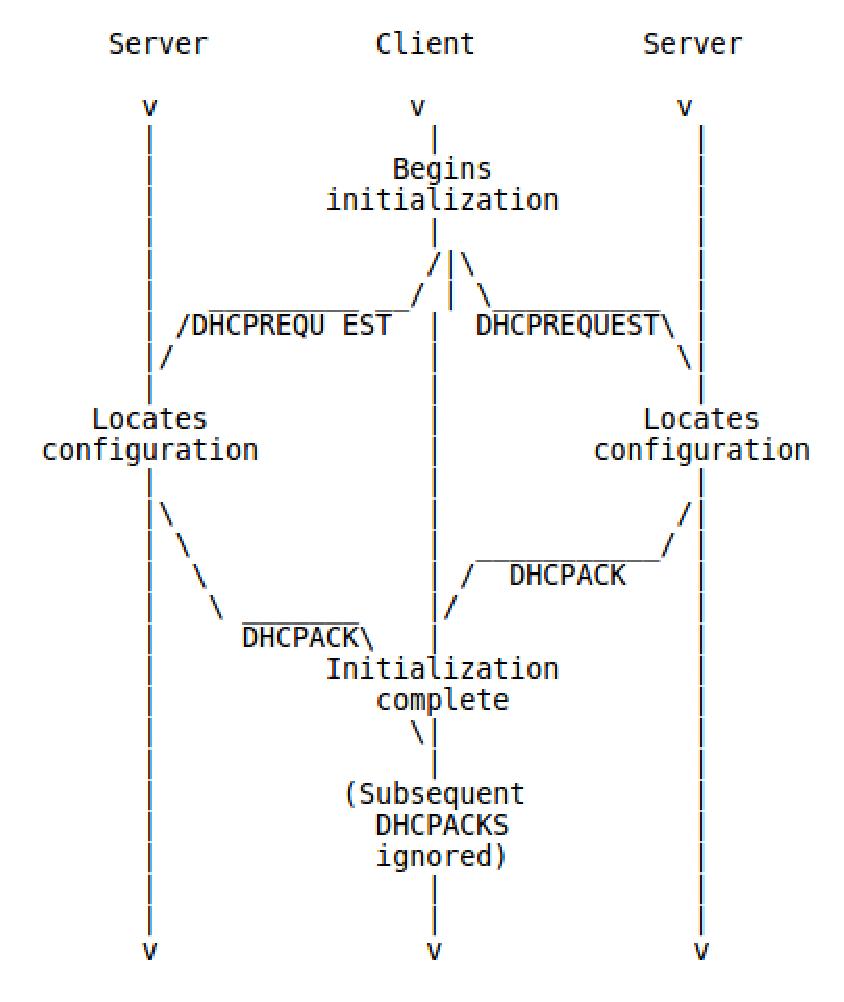
\includegraphics[width=6cm]{./pics/timeline_dhcp_reuse_add.eps}


\section{Passage de IPv4 à IPv6}
\subsection{Raison du passage de IPv4 à IPv6}
\subsubsection{Problème posé par IPv4}
//Pénrurie, adressage privé/publique compliqué
% Il se trouve que apparement il y a des problemes de
% penurie d'adresses meme dans certaines reseau prive`
% http://blog.erratasec.com/2013/12/dod-address-space-its-not-conspiracy.html#.WAf_d7Wf21F

PROBLÈMES DE IPV4

ÉPUISEMENT DES ADRESSES
Lorsque IPV4 a été développé dans les années 70-début des années 80, personnes n'aurait imaginé qu'il y aurait un jour autant d'interfaces qui se connectent à Internet. On pensait qu'une adresse sur 32 bits serait suffisante. De plus, les plages d'adresses étaient distribuées généreusement au début. Cela veut dire que l'on attribuait des adresses permettant un nombre d'interfaces beaucoup plus grand que nécessaire.
Cependant, avec la croissance du nombre d'utilisateurs, la plage d'adresses IPV4 disponible a diminué progressivement. C'est en février 2011 que la réserve de bloc libres d'adresses publics IPV4 de l'IANA (Internet Assigned Numbers Authority) est arrivée à épuisement.
Afin de résoudre ce problème, plusieurs techniques ont été proposées.
La première a été le changement de teechnique d'adressage. On est passé de la technique de classe d'adressage IP à la technique Classless Inter-Domain Routing. Ceci à permis une meilleure efficacité dans la distribution des adresses IP grâce à la création de réseau de tailles intermédiaire. En effet, avant on ne disposait que de réseau de 3 tailles différentes.
Les politiques d'assignement d'adresses ont également été rendu plus stricte afin de mieux tenir compte des besoin réels des demandeurs d'adresses IP.
Il a aussi été décidé d'utiliser des blocs autrefois réservé comme 14.0.0.0.
Sur base de volontarisme, des blocs autrefois attribués généreusement ou alors des IP non utilisées ont été récupérées. 
Finalement, il a été remarqué qu'il n'était pas nécessaire que chaque interface a son adresse IP public et le protocole NAT a été développé afin de regrouper plusieurs interface sous une même adresse IP. Ce protocole est de plus en plus utilisé dans IPV4 depuis la fin des années 90.

Fonctionnement du NAT dynamique (Network Adress Translation)
Le NAT est une technique utilisée au niveau du routeur. Le principe du NAT est que le routeur fait correspondre à une adresse IP une autre adresse IP. En général cette technique est utilisée pour avoir une même adresse IP pour tout un réseau comme un intranet ou encore un réseau domestique. Dans ce réseau, toutes les interfaces - même le routeur - auront une adresse privée. Le routeur dispose en plus de cela de une ou plusieurs adresses publics avec lesquelles il est connecté à internet. Une adresse privée est une adresse qui est utilisée à l'intérieur d'un réseau local. Les adresses privées peuvent être choisies parmi les suivantes : 10.0.0.0/8, 172.16.0.0/12 ou 192.168.0.0/16.
Lorsqu'une interface envoie un paquet vers l'extérieur du réseau, le routeur effectue plusieurs changements. Il traduit d'abord l'adresse privée en adresse public et la met dans l'en-tête du paquet. Puis il change tous les checksums qui tiennent compte de l'adresse IP. Enfin, il garde en mémoire dans une table la correspondance entre adresse privée/adresse public comme ci-dessous.
<tableau adresse public / privée >
Cela n'est cependant pas suffisant. En effet, lorsqu'un paquet arrivera de l'extérieur du réseau,  et si tous les interfaces utilisent la même adresse public sans distinction supplémentaire, le routeur ne saura pas à quelle interface envoyer le paquet. 
Une solution à ce problème existe pour les protocoles utilisant les ports comme TCP et UDP. Le routeur ajoute une information supplémentaire dans la table qui est le port source d'où vient le paquet. Les ports, qui sont implémentés dans la couche transport (couche 4), sont des sortes de ''portes'' qui permettent de communiquer avec un système d'exploitation. Le numéro de port est un numéro choisit aléatoirement entre 1024 et 65535.
Pour illustrer le fonctionnement du NAT imaginons qu'une interface A dont l'ip est 192.168.0.1 veut envoyer un paquet à l'interface B d'ip 217.70.184.38. Le port source est le port 10277 et le port destination est le port 80. 
La table NAT ressemblera à ceci : 

<TABLE NAT complète > 

La box internet enverra le paquet : 

L'interface B répondra en envoyant le paquet :

Lorsque la box reçoit ce paquet, elle voit que le port de destination est le port 10277. Elle cherche ensuite le port correspondant dans sa table NAT. Lorsqu'elle le trouve elle effectue les changements nécessaire sur le paquet et transmet le paquet à l'interface A.
Mais même si cette solution fonctionne la plupart du temps, la probabilité est faible que 2 interfaces envoient des paquet sur les même port. C'est pour éviter cela que la box change le port source lorsqu'elle reçoit un paquet de l'interface A. Ainsi on s'assure que aucun port n'est utilisé plusieurs fois. Enfin, pour éviter de saturer les ports utilisés, un compteur est associé à chaque paire adresse public/adresse privée. Lorsqu'il n'y a pas de trafic entre une adresse privée et l'extérieur durant une durée fixée, le port qui lui est associée peut être réutilisé pour une autre adresse privée.

Le NAT dynamique apporte cependant un grand problème. Lorsqu'une interface extérieur veut se connecter à une interface dans le réseau, elle ne dispose d'aucune autre information que l'adresse IP public. Si elle envoie alors un paquet à cette adresse, le routeur qui le réceptionnera ne saura pas quoi faire avec et le paquet sera perdu. 
 On a réussi à pallier à ce problème grâce au port forwarding. 

PORT FORWARDING

NAT STATIQUE


\subsubsection{Solutions}
//NAT,IPv6
\subsection{Différence entre IPv4 et IPv6}

\section{Conclusion}
\label{sec:ccl}

\addcontentsline{toc}{section}{Références}
\bibliographystyle{plain}
\bibliography{rapport}

\end{document}
